\documentclass[12pt]{article}
\usepackage[noblocks]{authblk}
\usepackage{graphicx}

\title{Comparative analysis of Gene Finding tools                                                                         
  when applied to \textit{Trichoderma} genomes} \author{Connor
  Burbridge} \affil{USask NSID: cbe453 \\ USask ID no.\ 11162928
  \\ Supervisors: Dave Schneider \& Tony Kusalik\\}

\begin{document}
\parindent=14pt
\maketitle

\clearpage
\section{Permission stuff}

\clearpage
\section{Abstract}

\clearpage
\section{Acknowledgements}

\clearpage
\tableofcontents

\clearpage
\section{Background}

\subsection{Trichoderma}

Crop resistance to environmental stressors is a necessity for crop
health and overall crop yields. Current popular methods for crop
protection involve the use of pesticides and genetically modified
organisms, which can be expensive and potentially politically dividing
in the case of GMOs\cite{GMO}. In addition, crops suffer when soils
are not sufficient for crop growth and health. Soil insufficiencies
can result in drought stress as well as nutrient stress, leading to
poor overall yields.

\textit{Trichoderma} is a type of fungi that can colonize the roots of
plants in a non-toxic, non-lethal, opportunistic symbiotic
relationship\cite{Trichoderma}. Many strains of \textit{Trichoderma}
have been shown to provide resistance to bacteria and other fungi in
soils through the use of polyketides, non-ribosomal peptide
synthetases and other antibiotic
products\cite{Trichoderma}\cite{Secretome}. Recently, two strains of
\textit{Trichoderma} have been identified in the prairie regions of
Alberta and Saskatchewan. These two strains, named Tsth20 and DC1,
have been found to have beneficial properties when used as an
inoculant for plants in the soils mentioned before. In addition to
these beneficial properties, the two strains mentioned previously
provide even further protection for plants in dry, salty soils and one
strain also has potential for use as a bioremediation tool in soils
contaminated with hydrocarbon content. Bioremediation and resistance
to drought tolerance has also been investigated in other strains of
\textit{Trichoderma} as well\cite{Drought}\cite{Kaminskyj}. However,
little is known about the mechanisms at work in these strains, so DC1
and Tsth20 were sequenced by the Global Institute for Food Security
(no publication yet) in an initial attempt to better understand the
details of these genomes. While this research does not directly
identify genomic elements related to the secretome of these genomes,
it may serve as a foundation for future research of
\textit{Trichoderma}.

\subsection{Genome Assembly}

Sequence assembly has been a long-standing application problem in the
field of bioinformatics\cite{assembly}. Determining the correct order
and combination of smaller subsequences into an accurate complete
sequence assembly is computationally difficult in terms of compute
resources such as memory, CPU cycles and storage required for input
sequences\cite{assembly}. In addition to these difficulties, there can
be other issues encountered during asssembly due to the nature of the
data or genomes themselves, such as low quality base calls for long
read data or the inherent content of genomes themselves using
repetitive regions as an example. Insufficient data used in an
assembly may result in short, fragmented assemblies, depending on the
size of the genomes, while sequence data that is not long enough can
fail to fully capture repetitive regions in an assembly. To solve this
problem, a wide range of assembly tools have been developed with their
own unique approaches to the genome assembly problem, so it is
important to use an appropriate assembler for the task at hand, and
also important to evaluate the assembly thoroughly. One approach to
aid in the previously mentioned issue of assembly correctness is to
use a combination of long and short reads in what is known as a hybrid
assembly. Combining both highly accurate short reads with deep
coverage along with less accurate but much longer reads can produce
high quality genome assemblies that capture long repetitive
regions. Hybrid assembly approaches have been shown to produce high
quality assemblies in a wide variety of organisms as the combine long
read data with short data to produce assemblies that properly
represent long repetetive regions with additionaly high quality
Illumina sequences for correction. Once assembled, the sequences must
also be evaluated with measures such as N50, L50, coverage, average
contig length and total assembled length to ensure that the genomes
are well assembled, at least based on these
metrics\cite{assembly}. Following appropriate assembly protocols is
essential to the further success of a project as downstream processing
such as annotation depends on a high-quality assembly.

\subsection{Repeat Identification/Masking and Identification of AT-rich Genomic regions}
Repeat identification within assembled genomes is a problem that needs
to be considered during the genome annotation process. Regions with
long repeats can have a significant impact on genome assembly as well
as gene finding due to the limitation of short reads used in some
assemblies\cite{Repeats}. Short reads may be unable to bridge or cover
entire repeat regions within a genome, so it is important to consider
the use of long reads from technologies such as Nanopore or PacBio to
provide a complete picture of these regions when pursuing a new genome
assembly project. It is also possible for repetitive regions to
contain genes as well, making for an interesting investigation in
regards to \textit{Trichoderma}, as fungal genomes have been shown to
contain many repeat regions with a high concentration of A and T
nucleotides\cite{fungalrepeats}. Once these repetitive regions have
been identified, the genome could be masked to exlude these regions in
downstream processing if desired, as these regions may be poorly
assembled and may result in found genes that do not truly exist in
those regions. However, this may not be as common today, as repetetive
regions have been shown to contain genes as well\cite{dontMask}. This
may affect the gene finding process described later and may be an
interesting topic to look into considering the large number of
available gene finding programs.

\subsection{Gene Finding}
Gene finding is another long standing computational problem in
bioinformatics, which concerns itself with identifying potential genes
within genomes based on patterns or evidence considered by the gene
finding program. There are two common methods for gene finding, those
methods being \textit{ab initio} methods, where programs search for
patterns and gene structures, and similarity or evidence-based
searches, which use prior information such as RNAseq data, expressed
sequence tags and protein sequences to identify genes within a new
genome\cite{GeneFinding}. Complicating the process more is the
introduction of introns and alternative splicing in eukaryotes, making
it possible for one gene to have several possible transcripts at the
same locus. Examples of \textit{ab initio} methods include tools such
as GeneMark-ES\cite{GeneMarkES} and GlimmerHMM\cite{Glimmer}, while
evidence based methods include tools such as \\ Braker2\cite{Braker2},
which can incorporate existing data such as RNAseq, protein sequences,
etc. in gene prediction models.

As mentioned previously, long repeats and transposable elements can
cause issues for gene finding programs, making this an interesting
area of research, at least for fungal genomes such as
\textit{Trichoderma}. Fungal genomes are also interesting in the topic
of gene finding as there are few programs targeted directly at gene
finding in fungal genomes while organisms such as human, mouse, and
\textit{Arabidopsis} benefit from having many tools tested on them as
they are model organisms in the field, according to table 1 of Wang, Z
\textit{et al}\cite{GeneFinding}. How these different methods and
tools perform when applied to fungal genomes is an important
consideration as fungi have features that can benefit plant growth as
mentioned earlier.

There are also other aspects of gene finding tools that are important
to consider. These include features such as whether or not the gene
finders find non-coding RNAs, annotation of 5' and 3' UTR regions, and
in the case of ab-initio methods, the assumptions made by the
underlying models used for gene finding. These features and others can
influence a user's decision on which gene finding tool to consider and
will complicate comparative analysis of multiple gene finding tools.

\section{Platform and Software Installation}
(Possibly supporting materials or discussion)

\subsection{Platform}
All analysis was performed on the RSMI server hosted on Copercius at
the University of Saskatchewan. This server is equipped with 64 cores
in addition to 1.5 TB of memory. The server is running RedHat
Enterprise Linux 7 as of writing this thesis. All data is stored
either on datastore, or in the RSMI scratch space.

\subsection{NextDenovo and NextPolish Installation}
Installation of nextDenovo was straightforward. Simply download the
compressed tar file from their website and unpack it. NextDenovo
requires Python versions 2 and 3 along with a package called parallel
to aid in parallel processing of datasets. The parallel package was
installed using pip in the bioinformatics conda environment in the
scratch space of Copernicus. NextPolish was installed in a Python
environment by a member of the research computing team that manages of
our system. Assistance was required for this as the version of RHEL
used by the server introduces glibc version conflicts with Anaconda
when trying to install nextPolish. 

\subsection{RepeatMasker Installation}

The installation procedure was somewhat indepth, requiring
RepeatMasker configuration, which itself requires downloading an
appropriate repeat database (Dfam in this case, included with
RepeatMasker), installation of Tandem Repeat Finder (TRFM) and
installation of a sequence search tool, for which I chose HMMER from
the list of potential tools as we were generally familiar with its
use. The path to the installation of TRFM is required during
configuration along with the search tool of choice, a simple selection
of 4 tools that will have an autocompleted path in this case, since
HMMER is installed via anaconda.

\subsection{GeneMark-ES Installation}
GeneMark-ES was successfully installed by downloading and unpacking
the package from their website along with a key required for use.

\subsection{Braker2 Installation}
Braker2 was also successfully installed by a member of the research
computing team who has set up several modules including an
initialization script to get things up and running as well as create a
reloadable environment for use again in the future. Once the
environment has been loaded, one must load the Hisat2 module from
Compute Canada as well as an htslib module (more detail to come). Once
all modules are loaded, there are a few environemnt variables that
need to be set, those being AUGUSTUS\_CONFIG\_PATH and
TSERBA\_CONFIG(?figure this out). In addition, a software package named
TSEBRA from the same developers as Braker2 must be installed for
consolidating gene calls. The variables can be set within the
braker2.pl command, which have higher priority over environment
variables and probably makes things easier to track.

\section{Methodology}

\subsection{Methodology Overview}

The general methodology for this work is described in figure 1. Each
portion of this figure is discussed in detail in this section.

\begin{figure}
  \begin{center}
    \makebox[\textwidth][c]{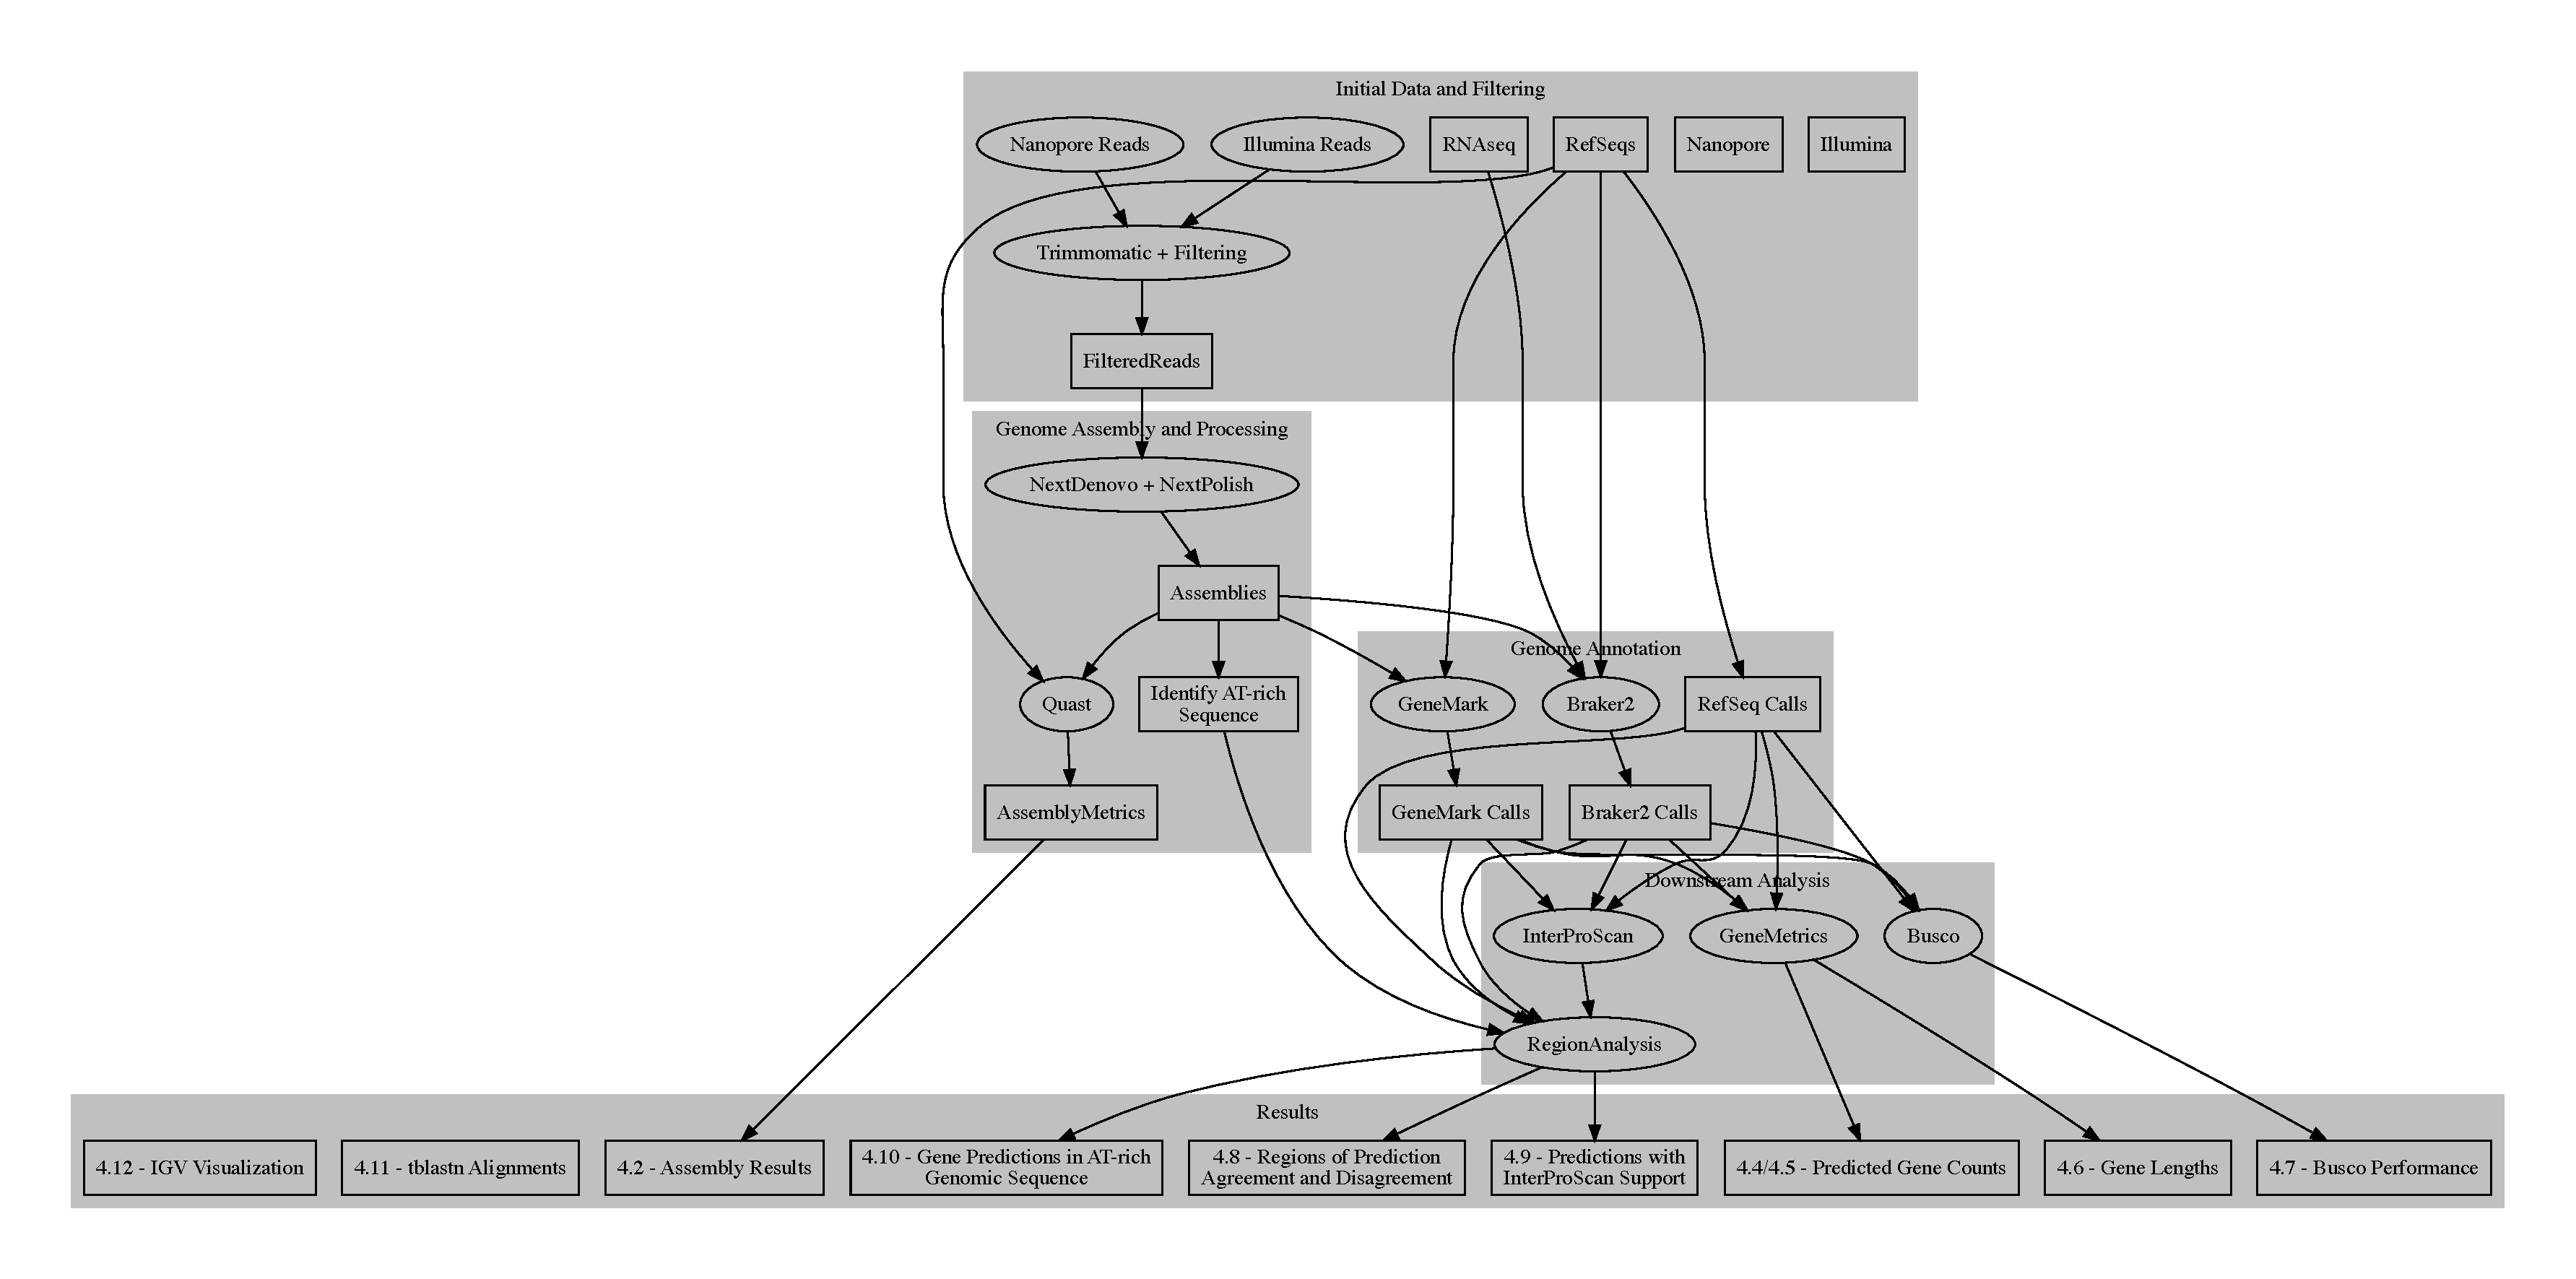
\includegraphics[width=1.4\textwidth]{./figures/data-flowchart.pdf}}%
  \end{center}
  \caption{A flowchart of the methodology followed for this
    research. Sections are separated based the general process they
    are associated with (i.e. input data, assembly, gene finding and
    downstream analysis).}
\end{figure}

\subsection{Selection of Existing \textit{Trichoderma} Genome Assemblies}

Comparing the performance and features, of gene finding tools, both
qualitative and quantitative, in the context of any set of genomes is
important for those interested in selecting a specific gene finding
tool. To accent(?) the processing for genomes of interest, those being
DC1 and Tsht20, we should include other previously assembled
\textit{Trichoderma} assemblies. Currently selected genomes include
\textit{Trichoderma reesei}, \textit{Trichoderma harzianum}, and
\textit{Trichoderma virens}, with \textit{Trichoderma reesei} being
the 'reference' in this case, as it is well studied and there are
several patents involving it's use a organsim for production of
compounds such as antibiotics in industrial applications.

\subsection{Assembly}

In an attempt to produce high quality assemblies of DC1 and Tsth20, We
decided on a set of tools named NextDenovo and NextPolish as they have
produced excellent assemblies based on previous experience. (should
find a citation to confirm this)

(Might be better for discussion or omitted since it is specific to our
setup) Initial attempts to run the example dataset resulted in
permissions errors due to the management of the storage system being
used, which were encountered with other tools in the past. To remedy
this, the software installation was copied to RSMI's scratch space on
Copernicus. Once the approriate permissions were given to run
nextDenovo, the example dataset was run without issue.

Following assembly using nextDenovo, Illumina sequence data from DC1
and Tsth20 was used to polish each respective genome using
nextPolish. Default parameters were used from assembly except for
modification of the parallel option to reduce processing times.

\subsection{Repeat Masking}

In order to evaluate the performance of gene finding tools in
repetitive or low complexity regions in the context of
\textit{Trichoderma} genomes, we must first identify said regions in
the genomes considered. To do this, RepeatMasker has been selected as
a tool to identify repeat regions based on a fungal subset of the Dfam
database by specifying the fungi species tag to RepeatMasker when
running the program. The program was configured with options to
produce several output formats for each genome considered, which will
allow for more informative downstream analysis of results. All
commands for repeat masking are located withing the processing
directory for each strain/genome.

(probably more suited for additional materials at the end?)
General command for running RepeatMasker:

/datastore/Roots/Connor/masters/software/repeatmasker/RepeatMasker/RepeatMasker
-pa 10 -a -small -species fungi -html -gff -dir ./
path-to-genome/genome.fasta

\subsection{GeneMark-ES}

To begin, GeneMark-ES was run as it requires no prior information or
alignments in order to run. In this case GeneMark-ES has an option
specifically for fungal genomes, which was used in this case. Apart
from the fungal option, the only additional options supplied were for
output format of GFF3 and number of cores for reduced processing time.

General command structure for GeneMark-ES:

gmes\_petap.pl --ES --fungus
--format gff3 --cores 48 --sequence /path/to/sequence

\subsection{Braker2}

As mentioned previously, \textit{Trichoderma reesei} was selected as
the \'reference\' genome for this work. With this in mind, several
short read archives (SRAs) from \textit{T. reesei} were selected for
Augustus training. Following Augustus training, the model for
\textit{T reesei} was applied to all genomes considered. Settings and
procedures from running Braker2 are described below.

The variables that need to be set are AUGUSTUS\_CONFIG\_PATH and
TSEBRA\_PATH. Augustus, by defuault, tries to write species
information to the location where the software is installed. In this
case, we don'thave write permissions to the compute canada software
stack hosted byt Research Computing, so the AUGUSTUS\_CONFIG\_PATH
variable must be set in order to create a writeable directory. As long
as that path has a directory within it called braker, and a species
directory within the braker directory, things should go
smoothly. TSEBRA is a set of scripts also made by the creators of
Braker and is required to merge results from the various gene
prediction tools involved in the Braker2 pipeline. The TSEBRA\_PATH
simply points to the directory where TSEBRA is located Both Braker2
and TSEBRA can be cloned directly from GitHub (links to come)

Example command for braker2:

/scratch/p2irc/p2irc\_rsmi/cbe453/masters/software/braker2/BRAKER/scripts/braker.pl
--gff3 --threads 60
--TSEBRA\_PATH=/scratch/p2irc/p2irc\_rsmi/cbe453/masters/software/braker2/tsebra/TSEBRA/bin/
--genome /path/to/sequence --species=TreeseiFungal --fungus
--useexisting

\section{Analysis of Results}

After completion of the processing portion of this work, the results
must be processed in a useful way, which includes both the biological
implications of the gene calls as well as the computational, or gene
finding features, of the the selected programs. To better understand
how gene finders perform in these two classes, we must define an
appropriate plan for analysis of the results produced so
far. Currently, downstream analysis plan has been broken down into
several sections.

\subsection{Basic Analysis}

Basic analysis of gene finding results is an important part of this
research. Total gene, transcript and protein counts will be identified
for each genome and gene finding tool combination. Comparing the
general outputs of these programs will provide an idea of their
performance in different \textit{Trichoderma} genomes In addition to
these basic outputs, analysis will also be performed for the
following: distribution of gene lengths, intersection of gene calls,
smallRNAs and repetetive regions, shared gene content with a close
fungal relative. Analysis for these results can be performed through
simple shell scripting with grep and other unix tools, although
processing through Python might provide results that are easier to
reproduce with proper programming. Having one script with several
modules that can be rerun at will would be easier to handle than
multiple shell scripts. This thinking for processing will be applied
to subsequent sections of this as well.

\subsection{Distribution of Gene Lengths}

One important aspect of gene finding tools to consider is the
distribution of gene lengths predicted by each individual
tool. Certain tools, such as GeneMark are based on pre-defined models,
which may limit the length of predicted genes, while tools such as
Braker2, which incorporate RNAseq data, may predict a wider
distribution of gene lengths depending on the input dataset
used. Regardless, the ability of a gene finding tool to predict a
wider range of gene lengths can be usefull if users are looking for
short or larger genes. To help determine whether or not these tools
find shorter genes, or small RNAs, the genomes of interest have been
annotated using Infernal along with the Rfam database to identify
small RNAs as a ground truth. These annotation results will also be
included with results from other annotation processes further down the
line. Again, these results can be produced with a Python script. The
resulting data could then be used as input to violin plots for each
genome and set of tools considered in this analysis process. Violin
plots should provide a good visualization of gene lengths as well as
the number of genes found with specific lengths. Means could also be
compared staatistically for genomes and the mutliple tools considered
as well.

Analysis of gene lengths was performed using a Python script. Combined
predicted CDS sequences for each predicted gene were used as input for
the total gene length. CDS sequences predicted by Braker2, were
directly available in the output directories when the program was
run. CDS sequences from GeneMark required extraction of the CDS
sequences from the genome FASTA files. This process was performed
using the gffread tool from the Cufflinks package. Predicted CDS
sequences were loaded into Python using Biopython's SeqIO
package. Sequence lengths were then placed in a list and analyzed
using a combination of pandas and numpy. A log10 transformation was
applied to the sequence lengths as the original distribution was
heavily skewed due to long outlier CDS sequences. After
transformation, the CDS length distribution appears as a normal
distribution, although there are interesting troughs that occur in
several of the peaks for several of the genomes considered. These
troughs did not appear in a comparable Yeast reference dataset,
although the log transformed data still appears to be a normal
distribution.

\subsection{Intersection of Gene Calls, smallRNAs and Repetitive Regions}

Annotation of all three features in the title are important in
assessing the ability of gene finding tools. Even more important, is
the potential for for overlap between gene calls and small RNAS as
well as repetitive regions the genomes. As discussed in the previous
subsection, the distribution of gene lengths predicted by a gene
finding tool can be an important metric for users. Overlapping
predicted genes from tools alongside the output from Infernal and the
Rfam database may provide insight into whether or not these gene
finding tools are able to predict RNAs of very short length. In
addition to small RNAs, repetitive regions in \textit{Trichoderma}
genomes hold potential for recombination and gene content, although
the inherent nature of these repetitive regions (low nucleotide
diveristy) suggests that gene content should be low, based on the
nucleotides required for start and stop codons. Analysis of these
intersections can be perfomed via bedtools or through biopython (I
believe). Again, having all processing steps included in one script as
separate functions that can be called at whim will make further
processing easier if changes need to be made.

\subsection{Methodology for Indetifying Overlapping Features}

To analyze the results from multiple gene-finding tools, we must first
define two conceptual topics.

Definition of a Feature: First, a feature, in the context of this
research, is any item contained within a Genomic Feature Formated file
(GFF). Each feature contains a contig ID, a start position, end
position, and a feature ID based on the information from the GFF
file. These features will be used in the process of identifying
regions, or overlapping features from prediction tools.

Definition of a Region: Secondly, a region is defined as any overlap
between features relative to the reference sequence being
considered. To identify regions, every feature from each GFF file
being considered, is sorted by start position. For clarification, the
start position is based on the left most position in the GFF file,
regardless of the strand that the feature is predicted on. Once the
features have been sorted by left position, the sorted features are
iterated over to identify regions, as long as the left position of the
next feature is consistent with the left position , within the left
and right position, or equal to the right position of the current
region. One drawback to this approach is that ideally, identification
of overlap types based on Allen's interval algebra would be performed
at this point. However, the methodology of initially sorting features
based on left position somewhat prevents this process from
happening. This implementation requires further processing of
identified regions late on the process, simplifying the all to all
comparison that would occurr if all features were considered at once.

\subsection{Shared Gene Content with Yeast}

While considering novel gene calls can be useful, comparing those
calls to a well-studied close relative can provide a rudimentary
validation of the calls as a ground truth. In this case, a comparison
to Yeast will be made. The agreed upon number for successful
gene-finding as compared to Yeast is roughly 80-85\% of gene
content. This will confirm that at least most of a closely related
fungal genome's content is predicted and shared by the gene calls for
\textit{Trichoderma}. Results for this processing can be produced with
a simple BLAST search and apropriate cutoff values (i.e. query
coverage, percent nucelotide identity, E-score, etc.). Other tools for
evaluation will certainly be considered, although I will need to look
into this process further.

\subsection{Comparative Genomics}

With the data produced by this research, it is possible to perform som
commparative genomics (time permitted), mostly related to the
assemblies generated during this work along with the RefSeq genomes
included from NCBI. Mummer is a potential tool to use for all to all
genome alignments, although there may be difficulty in the ordering of
contigs/scaffolds/chromosomes when performing thes alignments. This
work is not necessarily required but would be interesting from a
biological perspective to identify rearrangements, inversions and
such.

\section{Results}

\subsection{Assemblies of DC1 and Tsth20}

The table below displays results from the assembly process using
nextDenovo and nextPolish in comparison to existing assemblies for
other \textit{Trichoderma} genome assemblies. \\

\begin{figure}
  \makebox[\textwidth][c]{
    \begin{tabular}{|c|c|c|c|c|c|c|}
      \hline
      Strain & Total Contigs & Total Length & Largest Contig & GC\% & N50 & L50 \\ \hline
      DC1 & 8 & 38.6 Mb & 11.49 Mb & 47.97 & 5.69 Mb & 3 \\ \hline
      Tsth20 & 7 & 41.58 Mb & 8.02 Mb & 47.33 & 6.52 Mb & 3 \\ \hline
      \textit{T. harzianum} & 532 & 40.98 Mb & 4.08 Mb & 47.61 & 2.41 Mb & 7 \\ \hline
      \textit{T. virens} & 93 & 39.02 Mb & 3.45 Mb & 49.25 & 1.83 Mb & 8 \\ \hline
      \textit{T. reesei} & 77 & 33.39 Mb & 3.75 Mb & 52.82 & 1.21 Mb & 9 \\ \hline
    \end{tabular}
  }
  \caption{Table of general assembly metrics produced by QUAST (a
    genome quality assement tool).}
  \label{table1} \vspace{0.5cm}
\end{figure}

\subsection{Initial Gene Finding Results}

\begin{figure}
  \makebox[\textwidth][c]{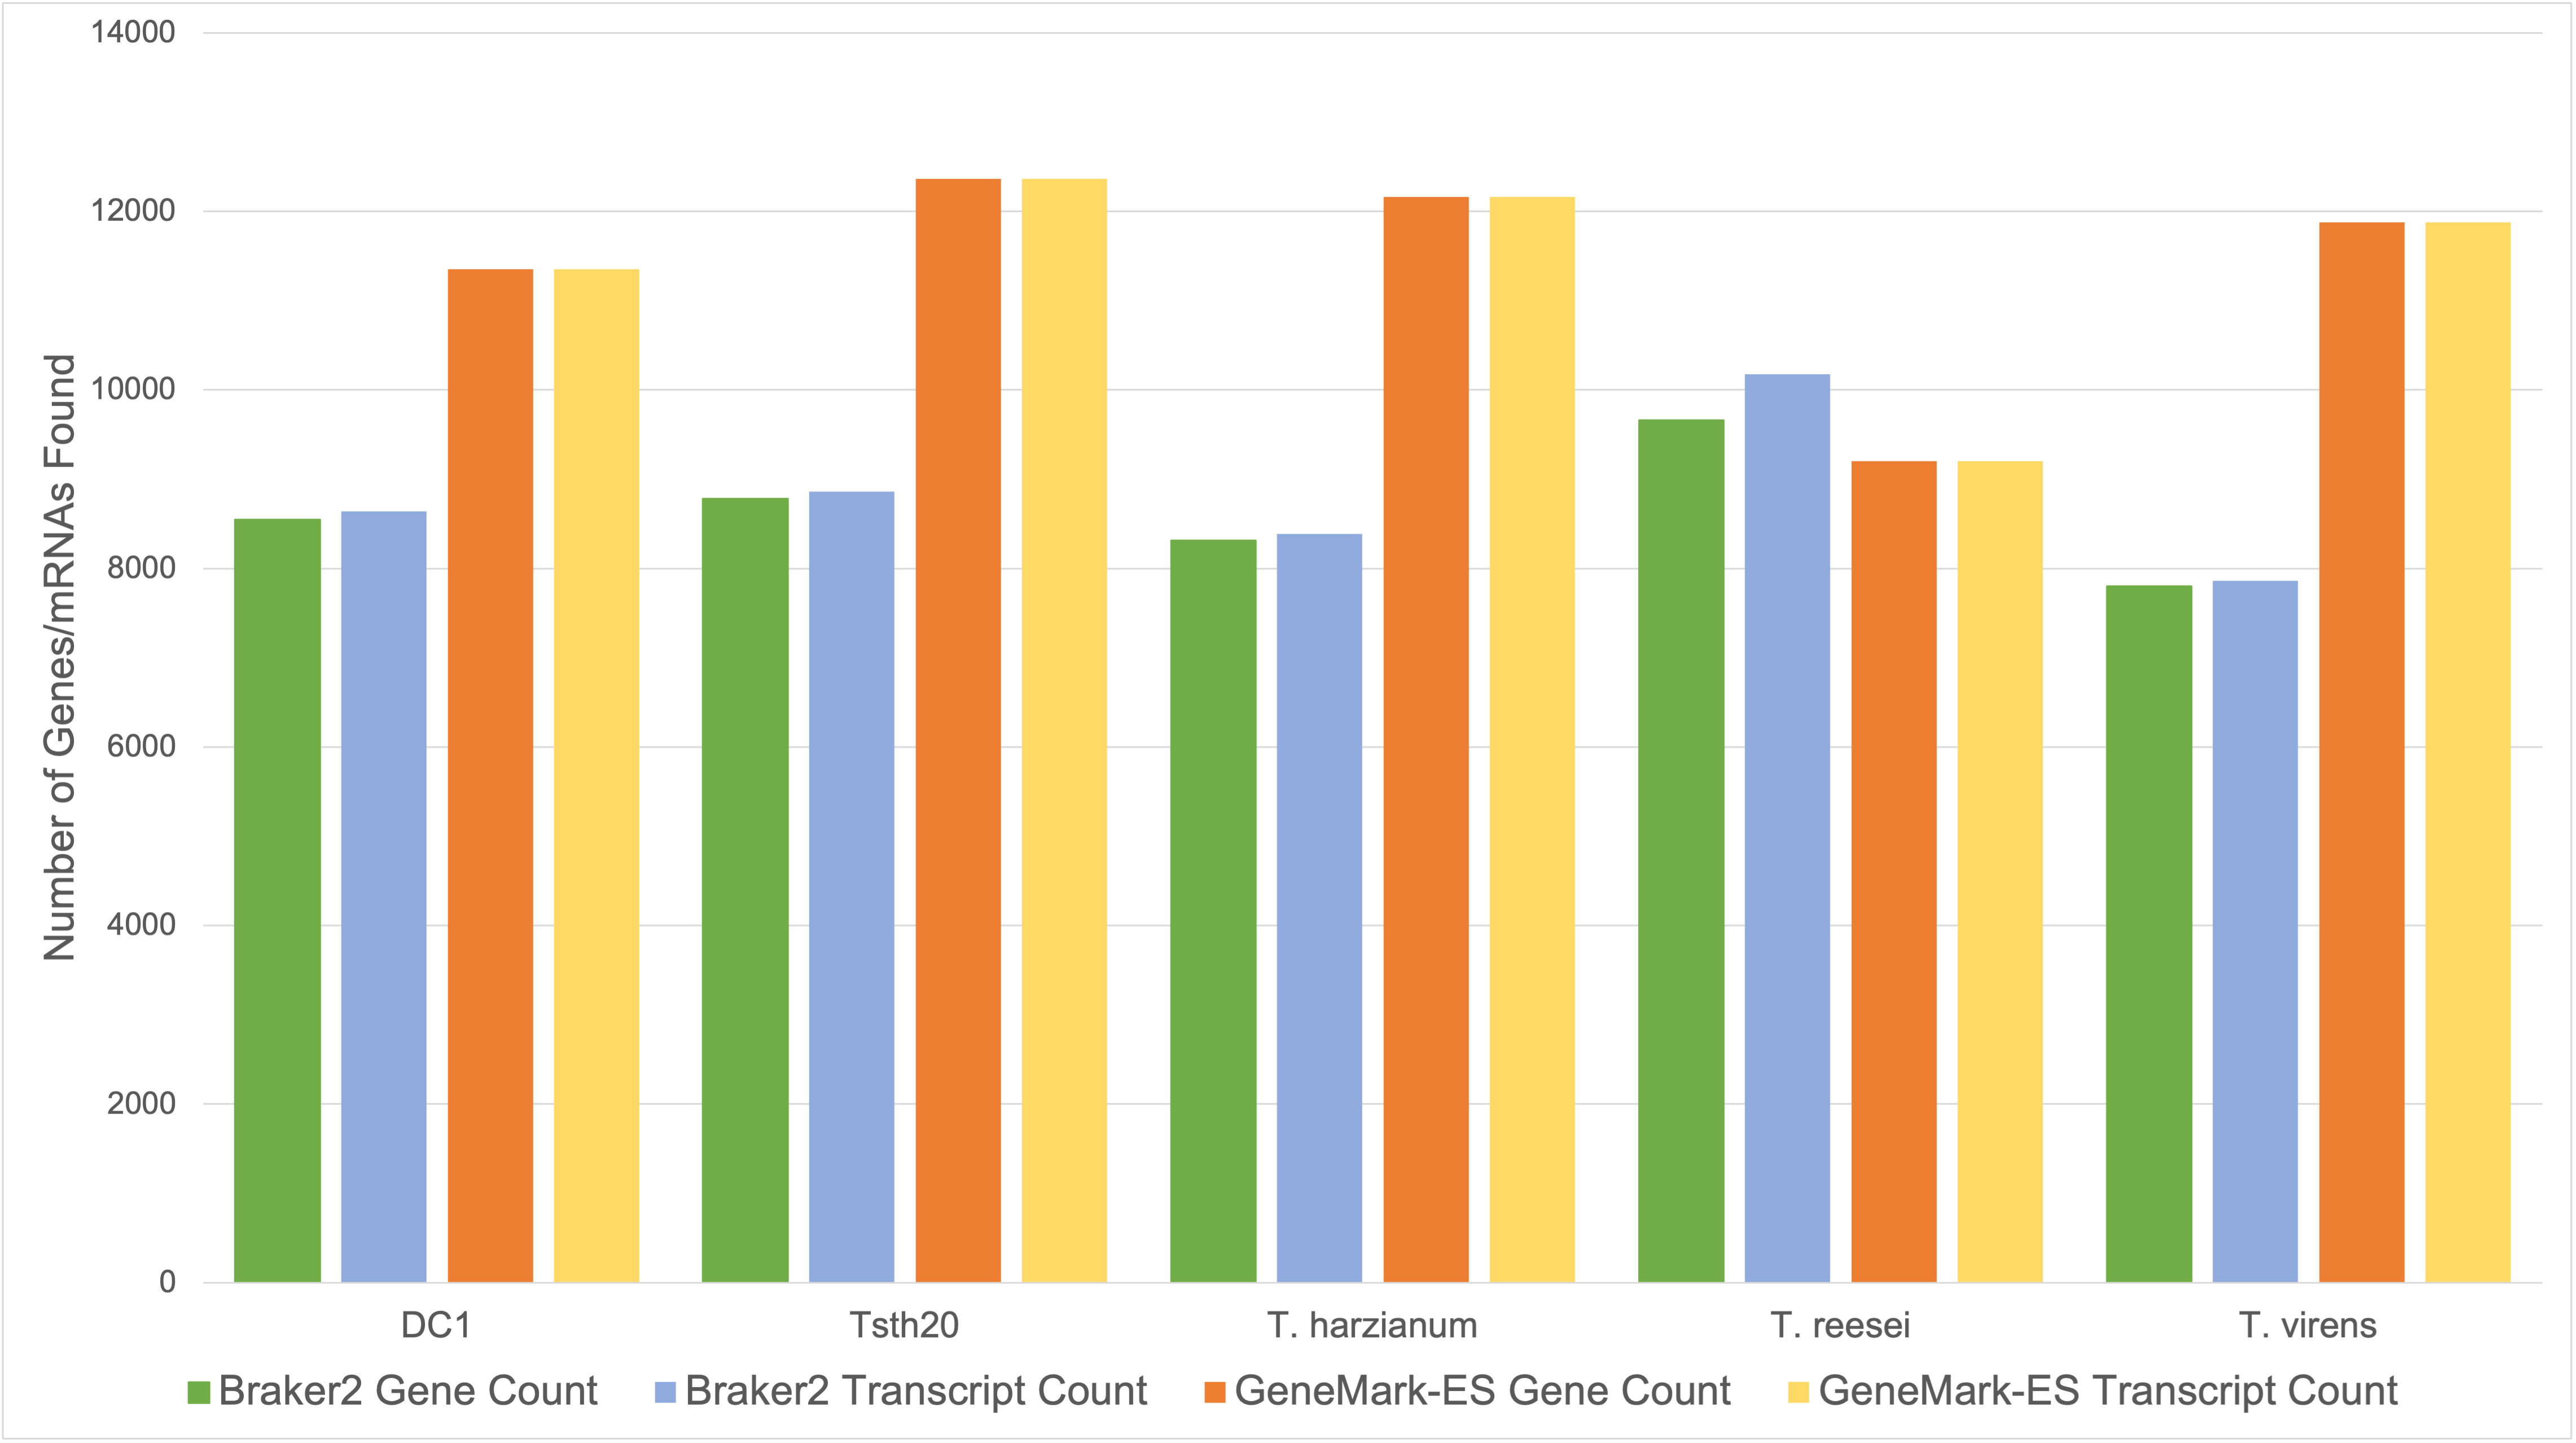
\includegraphics[width=1.2\textwidth]{./figures/nextpolish-gene-finding.png}}%
  \caption{Figure 3 shows the counts of genes and mRNAs found by each
    gene finding tool for each genome assembly considered.}
\end{figure}

\section{Discussion}

\section{Conclusions}

\clearpage

\section{References}
\begin{thebibliography}{99}
\bibitem{GMO} Zhang, C., Wohlhueter, R., Zhang, H. (2016). Genetically
  modified foods: A critical review of their promise and
  problems. \textit{Food Science and Human Wellness}, \textit{5}(3),
  116-123.

\bibitem{Trichoderma} Hermosa, R., Viterbo, A., Chet, I., Monte,
  E. (2012). Plant-beneficial effects of \textit{Trichoderma} and of
  its genes. \textit{Microbiology}. \textit{38},
  17-25. 

\bibitem{Secretome} Ramirez-Valdespino, C., Casas-Flores, S.,
  Olmedo-Monfil, V. (2019). \textit{Trichoderma} as a Model to Study
  Effector-Like Molecules. \textit{Frontiers in Microbiology}, \textit{15}.

\bibitem{Drought} Repas, T.S., Gillis, D.M., Boubakir, Z., Bao,
  Xioahui., Samuels, G.J., Kaminskyj, S.G.W. (2017). Growing plants on
  oily, nutrient-poor soil using a native symbitoic
  fungus. \textit{PLOS ONE}, \textit{12}(10).

\bibitem{Kaminskyj} Kaminskyj et al. (2012). Method for increasing
  plant growth using the fungus \textit{Trichoderma harzianum} (United
  States PCT/CA2O1O/OO1454). https://patentimages.storage.googleapis.com/57/4f/7f/5ff60c47045f01/US20120178624A1.pdf
  
\bibitem{Braker2} Hoff, K. J., Lomsadze, A., Borodovsky, M., Stanke,
  M. (2019). Whole-Genome Annotation with BRAKER. \textit{Methods Mol
    Biol.}, \textit{1962}, 65-95.

\bibitem{GeneMarkES} Borodovsky, M., Lomsadze, A. (2011). Eukaryotic
  Gene Prodeiction using GeneMark.hmm-E and
  GeneMark-ES. \textit{Current Protocols in
    Bioinformatics}. \textit{4}.

\bibitem{Glimmer} Majoros, W.H., Pertea, M., Salzberg, S.L. (2004) TigrScan and
  GlimmerHMM: two open-source \textit{ab initio} eukaryotic
  gene-finders. \textit{Bioinformatics}. \textit{20}(9), 2878-2879.
  
\bibitem{AUGUSTUS} Stanke, M., Morgenstern, B. (2005). AUGUSTUS: a web
  server for gene prediction in eukaryotes that allows user-defined
  constraints. \textit{Nucleic Acids Research}. \textit{33}, 465-467.
  
\bibitem{InterProScan} Jones, P., Binns, D., Chang, H. Y., Fraser,
  W., Li, W., Hunter, S. (2014). InterProScan 5: genome-scale
  protein function
  classification. \textit{Bioinformatics}. \textit{30}(9),
  1236-1240.

\bibitem{AnnotationSummary} Yandell, M., Ence, D. (2012). A beginner's
  guide to eukaryotic genome annotation. \textit{Nature Reviews
    Genetics}. \textit{13}, 329-342.
  
\bibitem{assembly} Sohn, J., Nam, J. (2016) The present and future of
  \textit{de novo} whole-genome assembly. \textit{Briefings in
    Bioinformatics}. \textit{19}1, 23-40.

\bibitem{spades} Bankevich, A., Nurk, S., Antipov, D., et
  al. (2012). SPAdes: a new genome assembly algorithm and its
  applications to single-cell sequencing. \textit{Joural of
    Computational Biology}. \textit{19}(5), 455-477. 
  
\bibitem{Repeats} Lerat., E. (2009). Identifying repeats and
  transposable elements in sequences genomes: how to find your way
  through the dense forest of programs. \textit{Nature
    Heredity}. \textit{104}, 520-533.

\bibitem{fungalrepeats} Li, WC., Huang, CH., Chen, CL. et
  al. (2017). Trichoderma reesei complete genome sequence,
  repeat-induced point mutation, and partitioning of CAZyme gene
  clusters. \textit{Biotechnol Biofuels}. \textit{10}, 170.

\bibitem{dontMask} Slotkin, R.K. (2018). The case for not masking away
  repetitive DNA. \textit{Mobile DNA}. \textit{9}(1), 15.
  
\bibitem{GeneFinding} Wang, Z., Chen, Yazhu., Li, Y. (2016). A Brief
  Review of Computational Gene Prediction Methods. \textit{Genomics
    Proteomics Bioinformatics}. \textit{2}4, 216-221.

\bibitem{RepeatMasker} Smit, A., Hubley, R., Green, P. (2013-2015)
  RepeatMasker Open-4.0. https://www.repeeatmasker.org

\bibitem{Infernal} Nawrocki, E.P., Eddy, S.R. (2013). Infernal 1.1:
  100-fold faster RNA homology
  searches. \textit{Bioinformatics}. \textit{29}, 2933-2935.

\bibitem{GenomeThreader} Gremme, G., Brendel, V., Sparks, M.E., Kurtz,
  S. (2005) Engineering a software tool for gene structure prediction
  in higher organisms. \textit{Information and Software
    Technology}. \textit{47}, 965-978.

\bibitem{Validation} Adav, S.S., Sze, S.K. (2014). Chapter 8 -
  \textit{TRichoderma} Secretome: An Overview. \textit{Biotechnology
    and Biology of Trichoderma}. 103-104. 
  
\end{thebibliography}

\end{document}
